\documentclass{article}
\usepackage[utf8]{inputenc}
\usepackage{graphicx}

\title{Relazione JFET}
\author{Francesco Pio Merafina, Onofrio Davide Caputo, Alessandro Lamesta}

\begin{document}

\maketitle

\section{Abstract:}
Lo scopo di questo esperimento è quello di verificare di poter usare un transitor di tipo JFET per poter creare un amplificatore, e poterne prevedere il comportamento mediante un modello teorico sviluppato precedentemente.
~
\section{Cenni teorici:}
Come il BJT il transistor JFET è composto da 3 cristalli e due giunzioni, ma lo schema circuitale ed il funzionamento è molto diversi, poichè il JFET ha entrambe le giunzioni polarizzate inversamente, entrambe collegate al gate (d'ora in poi indicato G), quindi in base alla tensione di G possiamo aumentare e diminuire la regione d'interdizione delle due giunzioni, inoltre considerando l'effetto della tensione tra drain e source (rispettivamente indicati con D ed S), otteniamo un effetto complessivo di potenziometro elettronico, infatti possiamo regolare la corrente che scorre usando la tensione G. Il JFET presenta più parametri di funzionamento rispetto al BJT, infatti abbiamo una tensione di pinchoff, cioè quella tensione di G tale per cui non può più scorrere corrente, una corrente di saturazione che si misura a tensione di G nulla e che è indipendente dalla tensione DS. Passando al comportamento in AC abbiamo due parametri dei quali tener conto, la transconduttanza tra D ed S e la resistenza r$_{d}$ che si presenta in parallelo ad un generatore ideale di corrente tra D ed S.
~
\begin{figure}[h!]
    \centering
    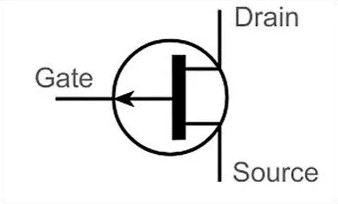
\includegraphics[width=\linewidth]{jfet.jpg} 
    \caption{Simbolo circuitale del JFET}
    \label{figura1}
\end{figure}
~
\begin{figure}[h!]
    \centering
    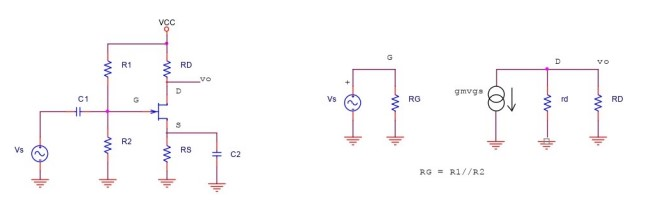
\includegraphics[width=\linewidth]{schemi amplificatore jfet.jpg} 
    \caption{Schema di montaggio dell'amplificatore JFET, e modellizzazione teorica dell'amplificatore}
    \label{figura1}
\end{figure}
~
\section{Strumentazione:}
La strumentazione usata consiste in:
\begin{itemize}
    \item Transistor JFET 2N3819
    \item le seguenti resistenze: 2 da 100K$\Omega$, 1 da 4.7K$\Omega$, 1 da 1K$\Omega$
    \item 3 condensatori da 47$\mu$F
    \item oscilloscopio
    \item generatore di tensione continua
    \item generatore di tensione alternata
\end{itemize}
Il tutto è  stato montato su basetta millefori con stagno e saldatore.
~
\section {Metodologia sperimentale e risultati:}
Prima di procedere con il montaggio del circuito si devono misurare i parametri I$_{dss}$, e V$_{gsoff}$, che vanno misurati con il transistor scollegato, per misurare I$_{dss}$ usiamo un amperometro e, a G chiuso, variamo la corrente fino a quando la corrente letta non è saturata, mentre per V$_{gsoff}$ usiamo l'amperometro come lettore di zero, aumentiamo la tensione di G fino a quando non leggiamo più corrente sull'amperometro.
~
\begin{figure}[h!]
    \centering
    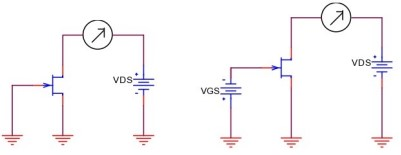
\includegraphics[width=\linewidth]{idss e vgsoff.jpg} 
    \caption{Schemi di misura per I$_{dss}$ e V$_{gsoff}$}
    \label{figura1}
\end{figure}
~
I valori sperimentali ottenuti delle due grandezze sono:
\begin{itemize}
    \item I$_{dss}$=5.5$\pm$0.5mA
    \item V$_{gsoff}$=0.904$\pm$0.005mV
\end{itemize}
noti questi valori possiamo ora ricavare quelli teorici del punto del punto di lavoro, e confrontarli con quelli sperimentali:
\begin{table}[]
    \begin{center}
        \begin{tabular}{c|c|c|}
         &Teorico&Sperimentale\\
      I$_{DS}$&1.37mA&1.35$\pm$0.05mA\\
      V$_{DS}$&4.08V&4.10$\pm$0.02V\\
      V$_{GS}$&-0.45&-0.45$\pm$0.05V\\
      \end{tabular}
   \end{center}
\end{table} 
Dopo aver concluso l'analisi DC, possiamo passare a quella AC, misurando la banda di guadagno, il guadagno effettivo e le resistenze di input ed output:
\begin{equation}
    R_i=(53.1\pm3.0)K\Omega   ;   R_o=(0.89\pm0.07)K\Omega
\end{equation}
E da qui, sapendo la relazione che lega la R$_{o}$, la R$_{D}$, e la r$_{D}$ possiamo ottenere la r$_{D}$=21$\pm$1.30K$\Omega$.
~
\begin{figure}[h!]
    \centering
    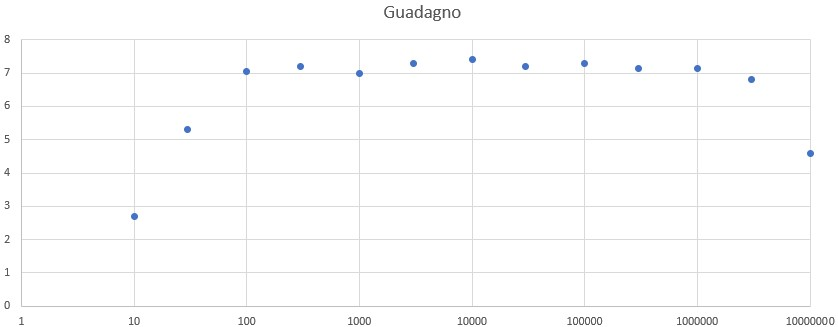
\includegraphics[width=\linewidth]{guadagno jfet.jpg} 
    \caption{Banda di guadagno}
    \label{figura1}
\end{figure}
~
\begin{table}[]
    \begin{center}
        \begin{tabular}{c|c|c|c}
        Frequenza[Hz]&V$_{i}$[mV]&V$_{o}$[mV]&Guadagno&\\
        10&51.0$\pm$2.0&140$\pm$5&2.75$\pm$0.15\\
        30&52.0$\pm$2.0&275$\pm$5&5.29$\pm$0.21\\
        100&51.5$\pm$2.0&357$\pm$5&6.93$\pm$0.23\\
        300&53.8$\pm$2.0&368$\pm$5&6.48$\pm$0.19\\
        1000&51.5$\pm$2.0&378$\pm$5&7.34$\pm$0.30\\
        3000&52.0$\pm$2.0&380$\pm$5&7.30$\pm$0.25\\
        10000&51.5$\pm$2.0&377$\pm$5&7.32$\pm$0.27\\
        30000&54.0$\pm$2.0&369$\pm$5&6.83$\pm$0.30\\
        100000&52.0$\pm$2.0&370$\pm$&7.12$\pm$0.16\\
        300000&50.0$\pm$2.0&374$\pm$5&7.48$\pm$0.25\\
        1000000&50.5$\pm$2.0&370$\pm$5&7.33$\pm$0.17\\
        3000000&52.0$\pm$2.0&354$\pm$5&6.81$\pm$0.18\\
        10000000&53.0$\pm$2.0&240$\pm$5&4.53$\pm$0.20\\
        \end{tabular}
   \end{center}
\end{table} 
~
Il guadagno teorico, ricavato dal modello corrisponde a 6.06, mentre quello sperimentale facendo una media pesata corrisponde a 7.12$\pm$0.10, ma possiamo comunque ritenere che il modello sia valido, poichè il valore teorico è stato ottenuto sulla base della misura di I$_{dss}$ e V$_{gsoff}$, in particolare la tensione di pinchoff è una misura molto delicata poichè usiamo un amperometro come misuratore di zero.
~
\section{Appendice:}
Testi di riferimento:
\begin{itemize}
    \item T. Floyd, Electronic devices, 9th ed. Prentice Hall
    \item Dell’Orso, Falchini, Flaminio et al. Introduzione all’elettronica digitale,
parte 2, Edizioni ETS, 2005

\end{itemize}





















\end{document}
